\documentclass[12pt, a4paper, font = Times New Roman]{article}
\usepackage[left= 3.5cm, top=3.5cm,bottom = 2cm, right=2cm]{geometry}
\usepackage{amsmath}
\usepackage{graphicx}
\usepackage{float}
\usepackage{subcaption}
\usepackage{url}
\usepackage{lipsum}


\begin{document}
\tableofcontents
\newpage
\listoffigures
\newpage

\section{Camera Calibration}

\subsection{Theory}
\par
Camera technology has experienced unprecedented research and development in modern times. Due to the high demand and mass production, there has been production of cameras with cheap and uncalibrated camera lenses. These issues has conclusively led to problems such as distortion of the images; primarily radial and tangential distortion.
\par
It has been identified that these distortion parameters are constant and can therefore be corrected for by using some mathematical manipulation.  
\par
The approach used for the calibration of IR camera in our project is discussed here. We consider the pinhole camera model approach which is depicted in the figure below.

\begin{figure}[h!]
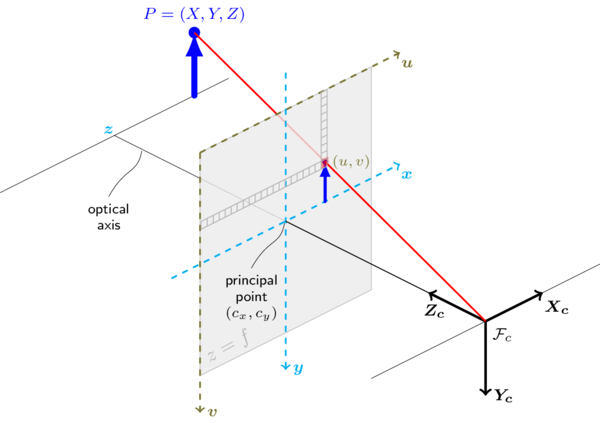
\includegraphics[scale=0.5]{pinhole_camera_model.png}
\caption{Pinhole camera model}
\label{fig:pinhole camera}
\end{figure}

\vspace{2cm}
\par
In this model, a scene view is formed by projection of 3D points into the image plane using a perspective transformation.

\begin{equation}\label{eq:1}
	s m' = A[R|t]M'
\end{equation}

or

\begin{equation}\label{eq:2}
	s 
\left[\begin{matrix}
u\\
v\\
1
\end{matrix}\right] = 
\left[\begin{matrix}
f_x & 0 & c_x\\
0 & f_y & c_y\\
0 & 0 & 1
\end{matrix}\right]
\left[\begin{matrix}
r_{11} & r_{12} & r_{13} & t_1\\
r_{21} & r_{22} & r_{23} & t_2\\
r_{31} & r_{32} & r_{33} & t_3
\end{matrix}\right]
\left[\begin{matrix}
X\\
Y\\
Z\\
1
\end{matrix}\right]
\end{equation}

\begin{itemize}
\item where:
\begin{itemize}
	\item (X, Y, Z) are the coordinates of a 3D point in the world coordinate space.
	\item (u, v) are the coordinates of the projection point in pixels
	\item A is a camera matrix, or a matrix of intrinsic parameters
	\item (cx, cy) is a principal point that is usually at the image center
	\item fx, fy are the focal lengths expressed in pixel units.
\end{itemize}
\end{itemize}

Real lenses usually have some distortion, mostly radial distortion and slight tangential distortion. So, the above model is extended as:

\begin{equation}\label{eq:3}
\left[\begin{matrix}
x\\
y\\
z
\end{matrix}\right] = 
R
\left[\begin{matrix}
X\\
Y\\
Z
\end{matrix}\right]
+ t
\end{equation}

\begin{equation}\label{eq:4}
x^{'} = x/z
\end{equation}
\begin{equation}\label{eq:5}
y^{'} = y/z
\end{equation}

\begin{equation}\label{eq:6}
x^{''} = x^{'}(1+k_1r^1+k_2r^4+k_3r^6) + 2p_1x^{'}y^{'}+ p_2(r^2_2x^{'2})
\end{equation}

\begin{equation}\label{eq:7}
y^{''} = y^{'}(1+k_1r^1+k_2r^4+k_3r^6) + p_1(r^2_2y^{'2})+ 2p_2x^{'}y^{'}
\end{equation}

\begin{equation}\label{eq:8}
u = f_x * x^{''} + c_x
\end{equation}

\begin{equation}\label{eq:9}
v = f_y * y^{''} + c_y
\end{equation}

\vspace{2cm}
The distortion produced due to camera is shown in figure below.


\begin{figure}[H]
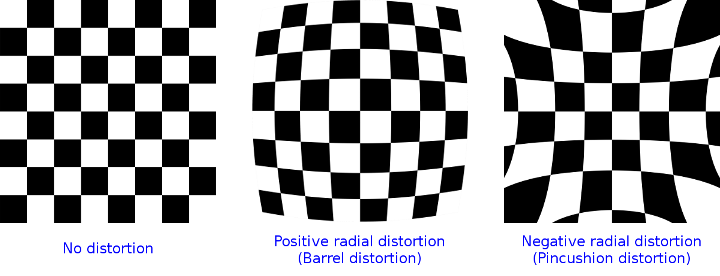
\includegraphics[scale=0.5]{distortion_examples.png}
\caption{Common camera distortion}
\label{fig:distortion}
\end{figure}

\vspace{2cm}

\subsection{Procedure}

\subsubsection{Setup}
\par
We have used functions provided by OpenCV inorder to perform calibration of camera. This requires taking multiple images of a chessboard pattern provided by OpenCV.
\par
We have used a chessboard pattern consisting of 9x6 cross-points. These cross-points are detected which provides 3D \emph{object points} and the corresponding 2D \emph{image points} are already stored. These points can now be applied to satisfy the equation \ref{eq:3} and the subsequent equations upto equation \ref{eq:9}. Solving the equations provide us with camera matrix, distortion matrix, rotational matrix and the translation matrix. These values can then be used to undistort the images taken with the uncalibrated camera.
\par
 Multiple images are to be taken of the chessboard to ensure sufficient accuracy.
\subsubsection{Algorithm}

Algorithm for camera calibration:
\begin{enumerate}
	\item Read the image files using $cv2.imread()$
	\item Convert into gray-scale using $cv2.cvtColor(image,cv2.COLOR\textunderscore BGR2GRAY)$
	\item Find the chessboard corners using $cv2.findChessboardCorners()$
	\item Refine the object points using $cv2.cornerSubPix()$
	\item Determine the camera matrix, distortion coefficients, rotation and translation vectors using $cv2.calibrateCamera()$
	\item Take the new image to be undistorted.
	\item Undistort the image using $cv2.undistort()$
\end{enumerate}

\subsubsection{Libraries}
Necessary libraries are listed below.
\begin{itemize}
\item OpenCV 3.0 library
\item Python compiler
\item Numpy library
\end{itemize}


\subsection{Results}
The result of camera calibration is shown below:

\begin{figure}[!h]
  \begin{subfigure}[b]{0.6\textwidth}
    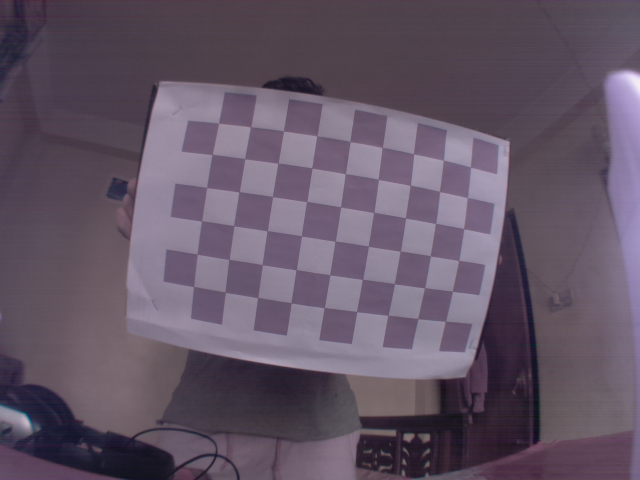
\includegraphics[width=\textwidth]{imagelack10000007.jpg}
    \caption{Original Image}
    \label{fig:original}
  \end{subfigure}
  \hfill
  \begin{subfigure}[b]{0.6\textwidth}
    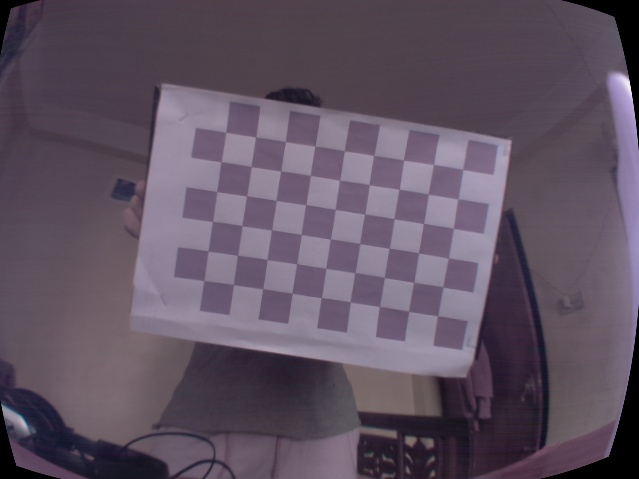
\includegraphics[width=\textwidth]{pqr.jpg}
    \caption{Undistorted image}
    \label{fig:undistorted}
  \end{subfigure}
  \caption{The effect of removal of distortion is clearly visible in the above comparison. The distorted image in the left is corrected in the image in right.}
\end{figure}
\clearpage

\newpage
\section{Image Enhancement Algorithms}

\par
Enhancement is done to restore an image that has gone through different kinds of deterioration due to environment, optics or any other factor. In this very project, image is taken at night time and hence has numerous noise and deterioration. For more efficient image capturing, IR camera has been used which up to some extent, gives us comparatively clearer image but not as needed. Hence, some image enhancement techniques need to be used in order to make the image clearer so that the object detection could be done with higher accuracy. Image enhancement is simply a process to improve the quality of image using different algorithms and processes. Hence, its purpose is to increase image visibility and details.



\begin{center}
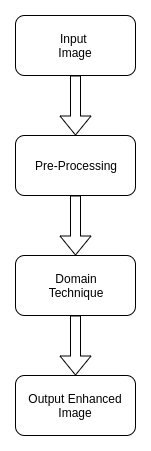
\includegraphics[scale=0.5]{Untitled_Diagram__2_.png}
\label{fig: Image_enhancement}
\captionof{figure}{Image Enhancement}
\end{center}

    \subsection{Histogram Equalization}
    \par
    Histogram of a image represents the numerical data of intensity and number of pixels corresponding to it. For example: the image with its histogram is shown below.

\begin{figure}[!h]
  \begin{subfigure}[b]{0.5\textwidth}
    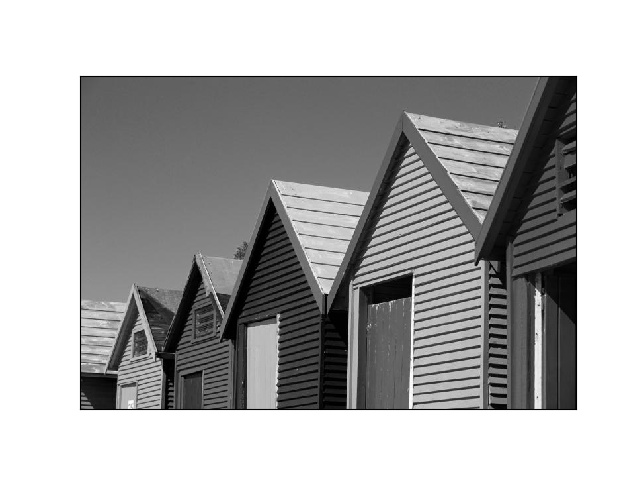
\includegraphics[width=\textwidth]{Orginal_bw.jpeg}
    \caption{Original Image}
    \label{fig:Orginal_bw}
  \end{subfigure}
  \hfill
  \begin{subfigure}[b]{0.5\textwidth}
    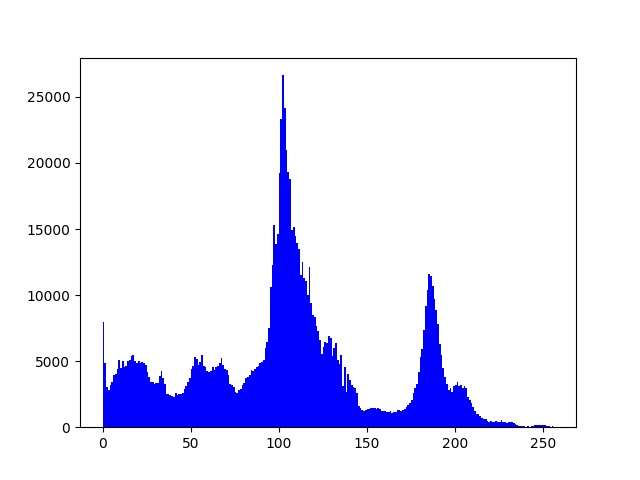
\includegraphics[width=\textwidth]{orginal_hist.jpeg}
    \caption{Histogram of Original Image}
    \label{fig:orginal_hist}
  \end{subfigure}
  \caption{The entropy of image in left is 5.09}
\end{figure}
\par
In histogram equalization, the CDF (Cumulative Distribution Function) of the pixel intensity is normalized in such a way that the new CDF becomes the linear function with constant slope. 
\par
CDF of the image can be determined as:

\begin{equation}
CDF(i) = \sum_{j=0}^{i}{P_x(j)}
\end{equation}
\par
Where,
\begin{equation}
P_x(i) = n_i/n
\end{equation}
\par
n represents the total number of pixels and $n_i$ is the number of pixels having same intensity i.
\par
\par
The original image has CDF as follows:

\begin{center}
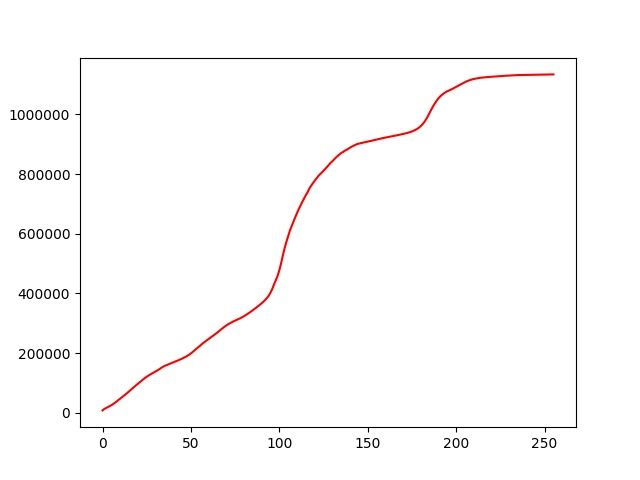
\includegraphics[scale = 0.4]{CDF_1.jpg}
\captionof{figure}{CDF of Original Image}
\label{CDF_1}
\end{center}

\par
Our goal of Histogram equalization is to recalculate the pixel intensity such that the new CDF is equal to the intensity(i) times any constant value(k).
\begin{equation}
CDF_new(i) = i*k
\end{equation}
\par
For that purpose, the pixels intensity has to be normalized as:
\begin{equation}
new_intensity(i) = round ( \frac{(df(i) - cdf_min)}{(no. of pixels -1)}  * (no. of intensity levels -1)
\end{equation}

\par
Now after histogram equalization, the result can be seen as:

\begin{figure}[!h]
  \begin{subfigure}[b]{0.5\textwidth}
    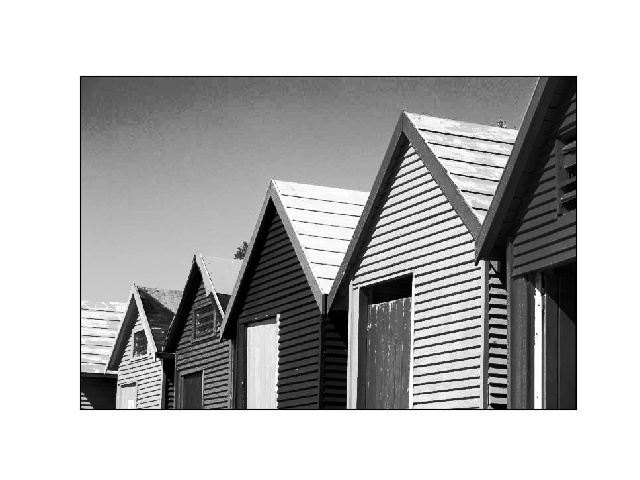
\includegraphics[width=\textwidth]{equalized_bw.jpeg}
    \caption{Histogram Equalized Image}
    \label{fig:equalized_bw}
  \end{subfigure}
  \hfill
  \begin{subfigure}[b]{0.5\textwidth}
    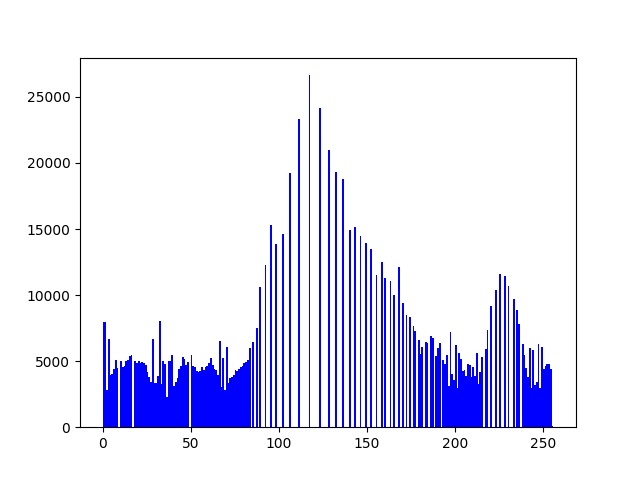
\includegraphics[width=\textwidth]{equalized_hist.jpeg}
    \caption{Histogram After Histogram Equalization}
    \label{fig:equalized_hist}
  \end{subfigure}
  \caption{The entropy of image in left is 5.34 which is greater than original image}
\end{figure}
The image has CDF:
\begin{center}
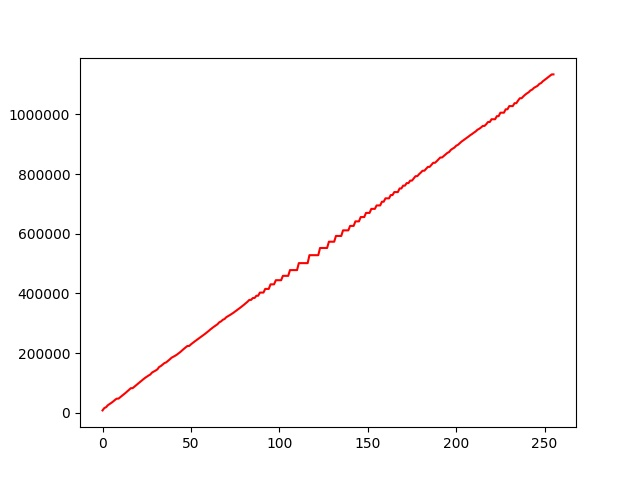
\includegraphics[scale = 0.4]{CDF_2.jpg}
\captionof{figure}{CDF of equalized image}
\label{CDF_2}
\end{center}

\clearpage
\newpage

\subsection{Adaptive Histogram Equalization (Entropy based)}
\par
In traditional approach to histogram equalization, the entropy of the result image is increased which causes loss of information. This approach suggested by Zhu and Hang in \cite{zhu_huang_2012} for histogram equalization preserves the entropy of the original image. There is an introduction of parameter $\beta$ and takes entropy content as target function.
Entropy content of an image is given as:
\begin{equation}
E = -\sum_{i=0}^{n-1}{p_ilogp_i}
\end{equation}

where $p(i)$ is the probability of occurrence of $i^{\text{th}}$ gray level.
\begin{equation}
p(i) = \frac{q_k}{Q}
\end{equation}

\subsubsection{Algorithm}
\par
$f_{\text{i}}$ is the gray value of $i^{\text{th}}$ gray level in the original image. Position j of the resultant image for corresponding $g_{\text{j}}$ of the original image is given by the transformation.

\begin{equation}
j = (m-1)\frac{\sum_{k=0}^{i-1}{p_k}}{\sum_{k=0}^{i-1}{p_k} + \sum_{k=i+1}^{m-1}{p_k}}
\end{equation}

\par
The parameter $\beta$ is introduced to prevent the gray-level with low number of pixels being overwhelmed by gray-level with large number of pixels in the neighborhood. the new transformation equation becomes:
\begin{equation}\label{eq:transform}
j = (m-1)\frac{\sum_{k=0}^{i-1}{p_k}}{\sum_{k=0}^{i-1}{p_k} + \beta \sum_{k=i+1}^{m-1}{p_k}}
\end{equation}
\paragraph{Selection of $\beta$:}
\par
For an 8-bit image with 256 gray-levels. It can be divided into 3 categories: low gray levels, middle gray level and high gray level. The threshold is set at TL=85, TH=170. The pixels at each of these categories are calculated and recorded.
\par
The maximum of the three is found and image type is determined.
\begin{itemize}
\item $\beta$ = 0.8 if number of pixel in low gray level is highest.
\item $\beta$ = 1.1 if number of pixel in medium gray level is highest.
\item $\beta$ = 1.5 if number of pixel in high gray level is highest.
\end{itemize}
\par
Although the algorithm has been only described for gray-scale image, this idea has been extended and used for all 3 channels\emph{(R,G,B)}. The steps for which is listed below:

\begin{enumerate}
\item Read the image.
\item Calculate the histogram for all 3 channels\emph{(R,G,B)}.
\item Normalize the histogram for \emph{(R,G,B)} channels.
\item determine $\beta$ for \emph{(R,G,B)} channels.
\item transform the image using \ref{eq:transform}.
\item Generate the new image.
\end{enumerate}





\subsubsection{Results}
\begin{figure}[!h]
  \begin{subfigure}[b]{0.5\textwidth}
    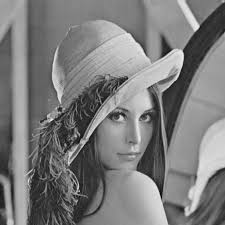
\includegraphics[width=\textwidth]{lena.jpg}
    \caption{Original Image}
    \label{fig:lena}
  \end{subfigure}
  \hfill
  \begin{subfigure}[b]{0.5\textwidth}
    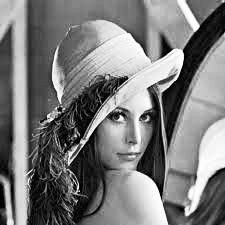
\includegraphics[width=\textwidth]{result_lena.jpg}
    \caption{Adaptive histogram equalized image}
    \label{fig:result_lena}
  \end{subfigure}
  \caption{The entropy of image in left is 7.466 and for image in right is 7.966}
\end{figure}


\begin{figure}[!h]
  \begin{subfigure}[b]{0.5\textwidth}
    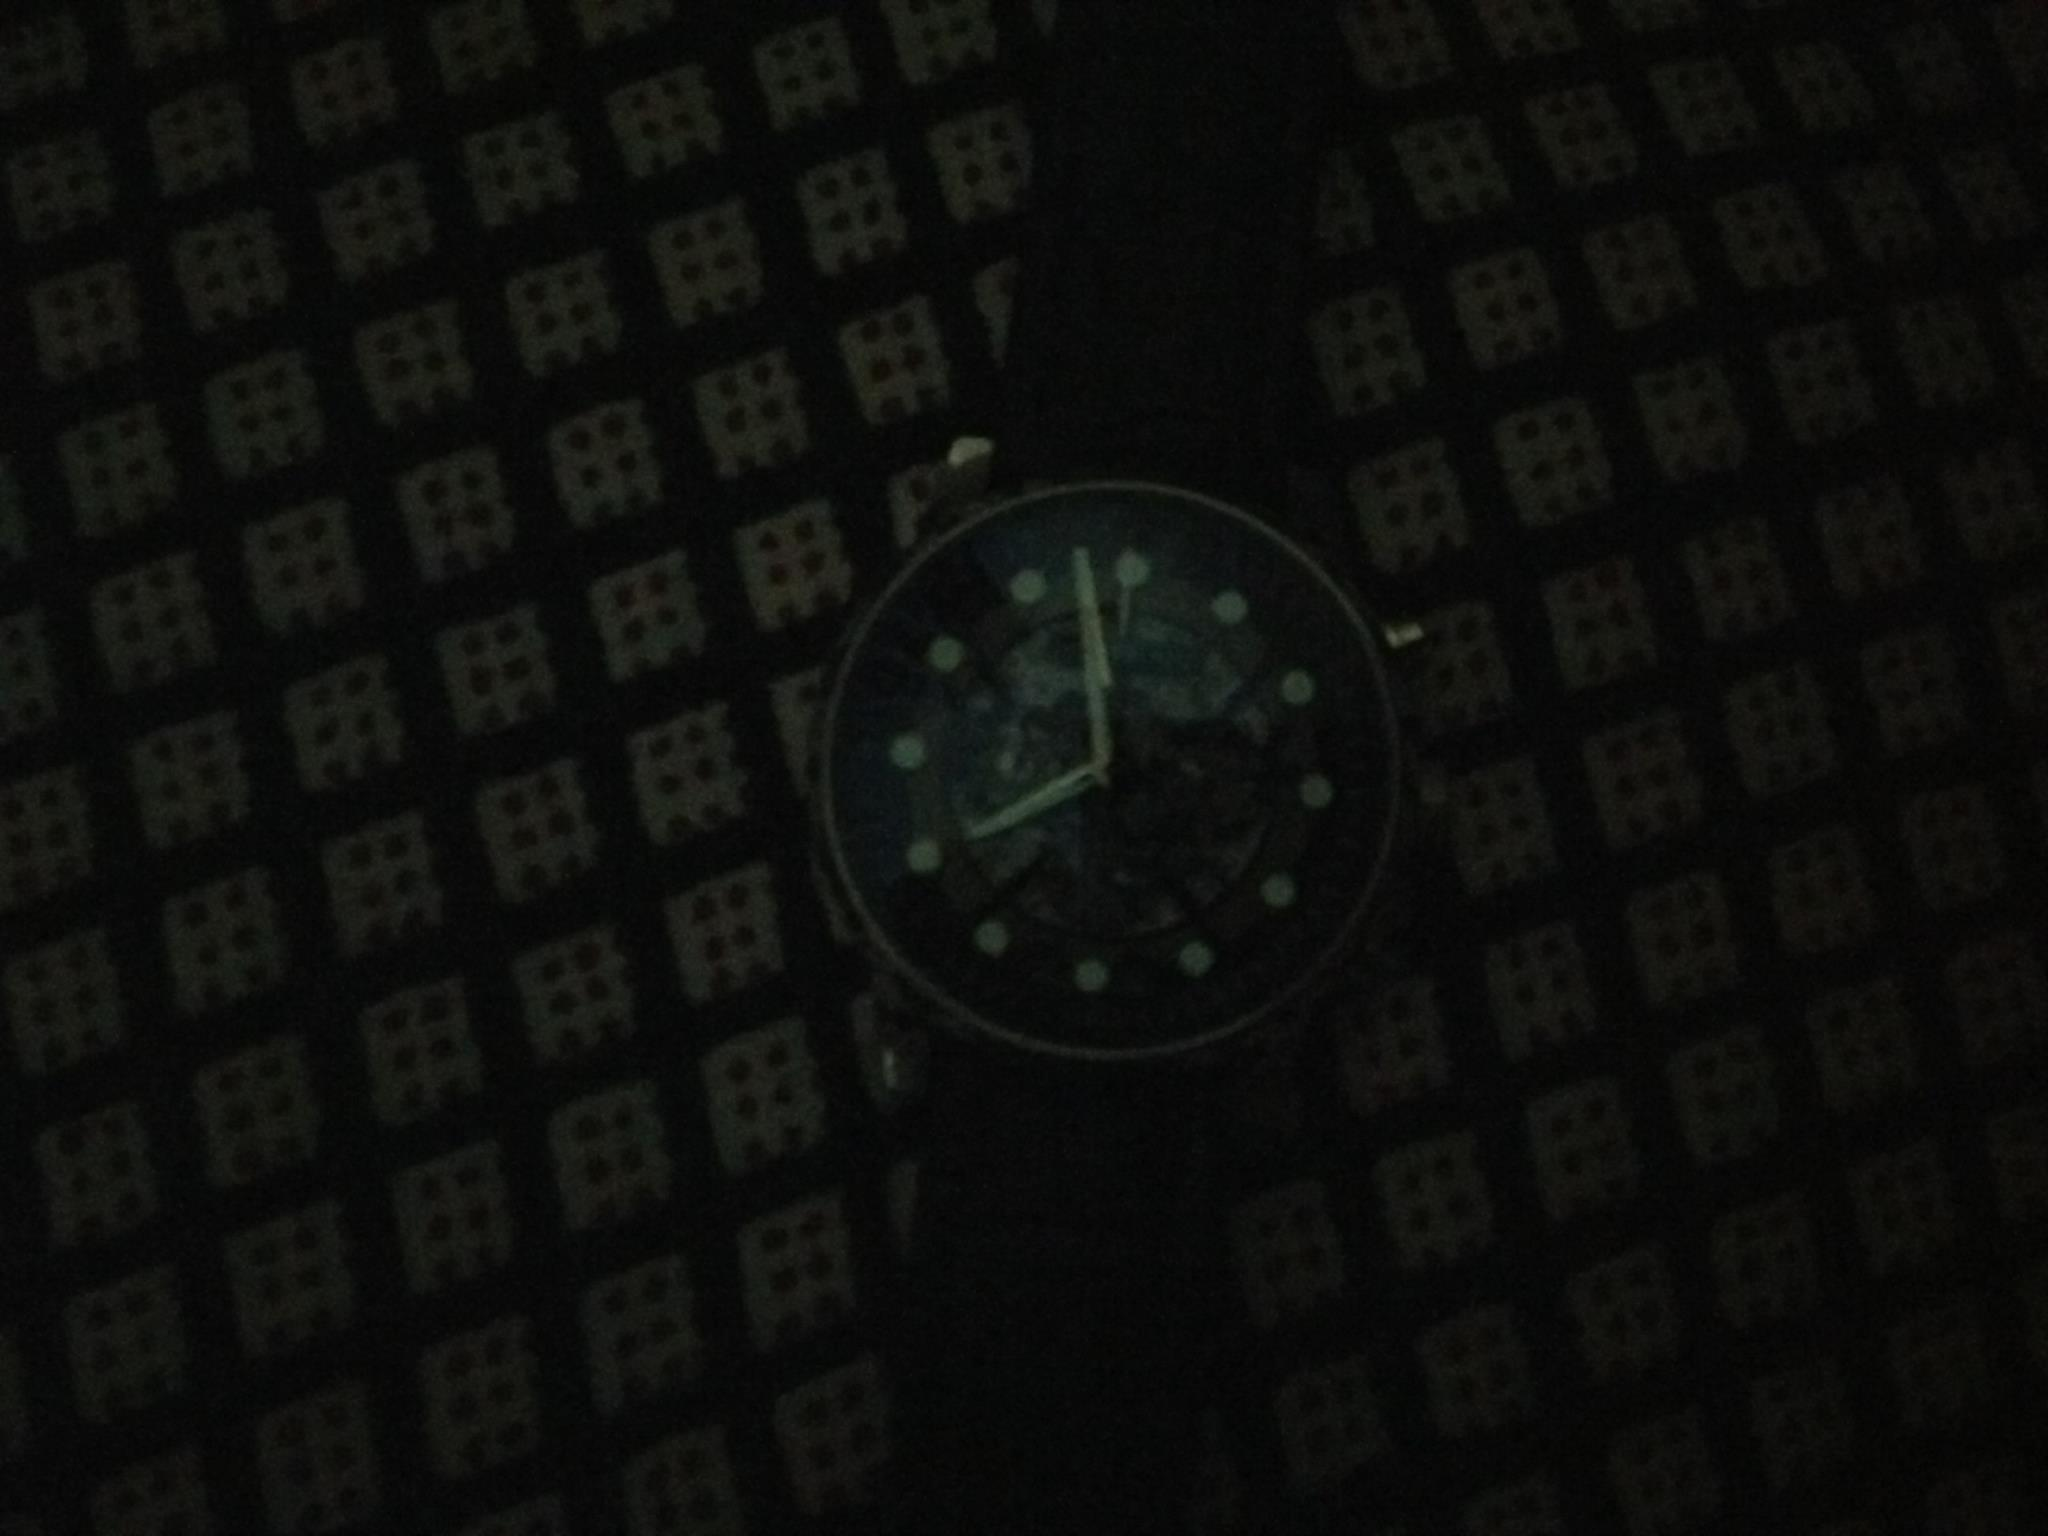
\includegraphics[width=\textwidth]{watch.jpg}
    \caption{Original Image}
    \label{fig:lena}
  \end{subfigure}
  \hfill
  \begin{subfigure}[b]{0.5\textwidth}
    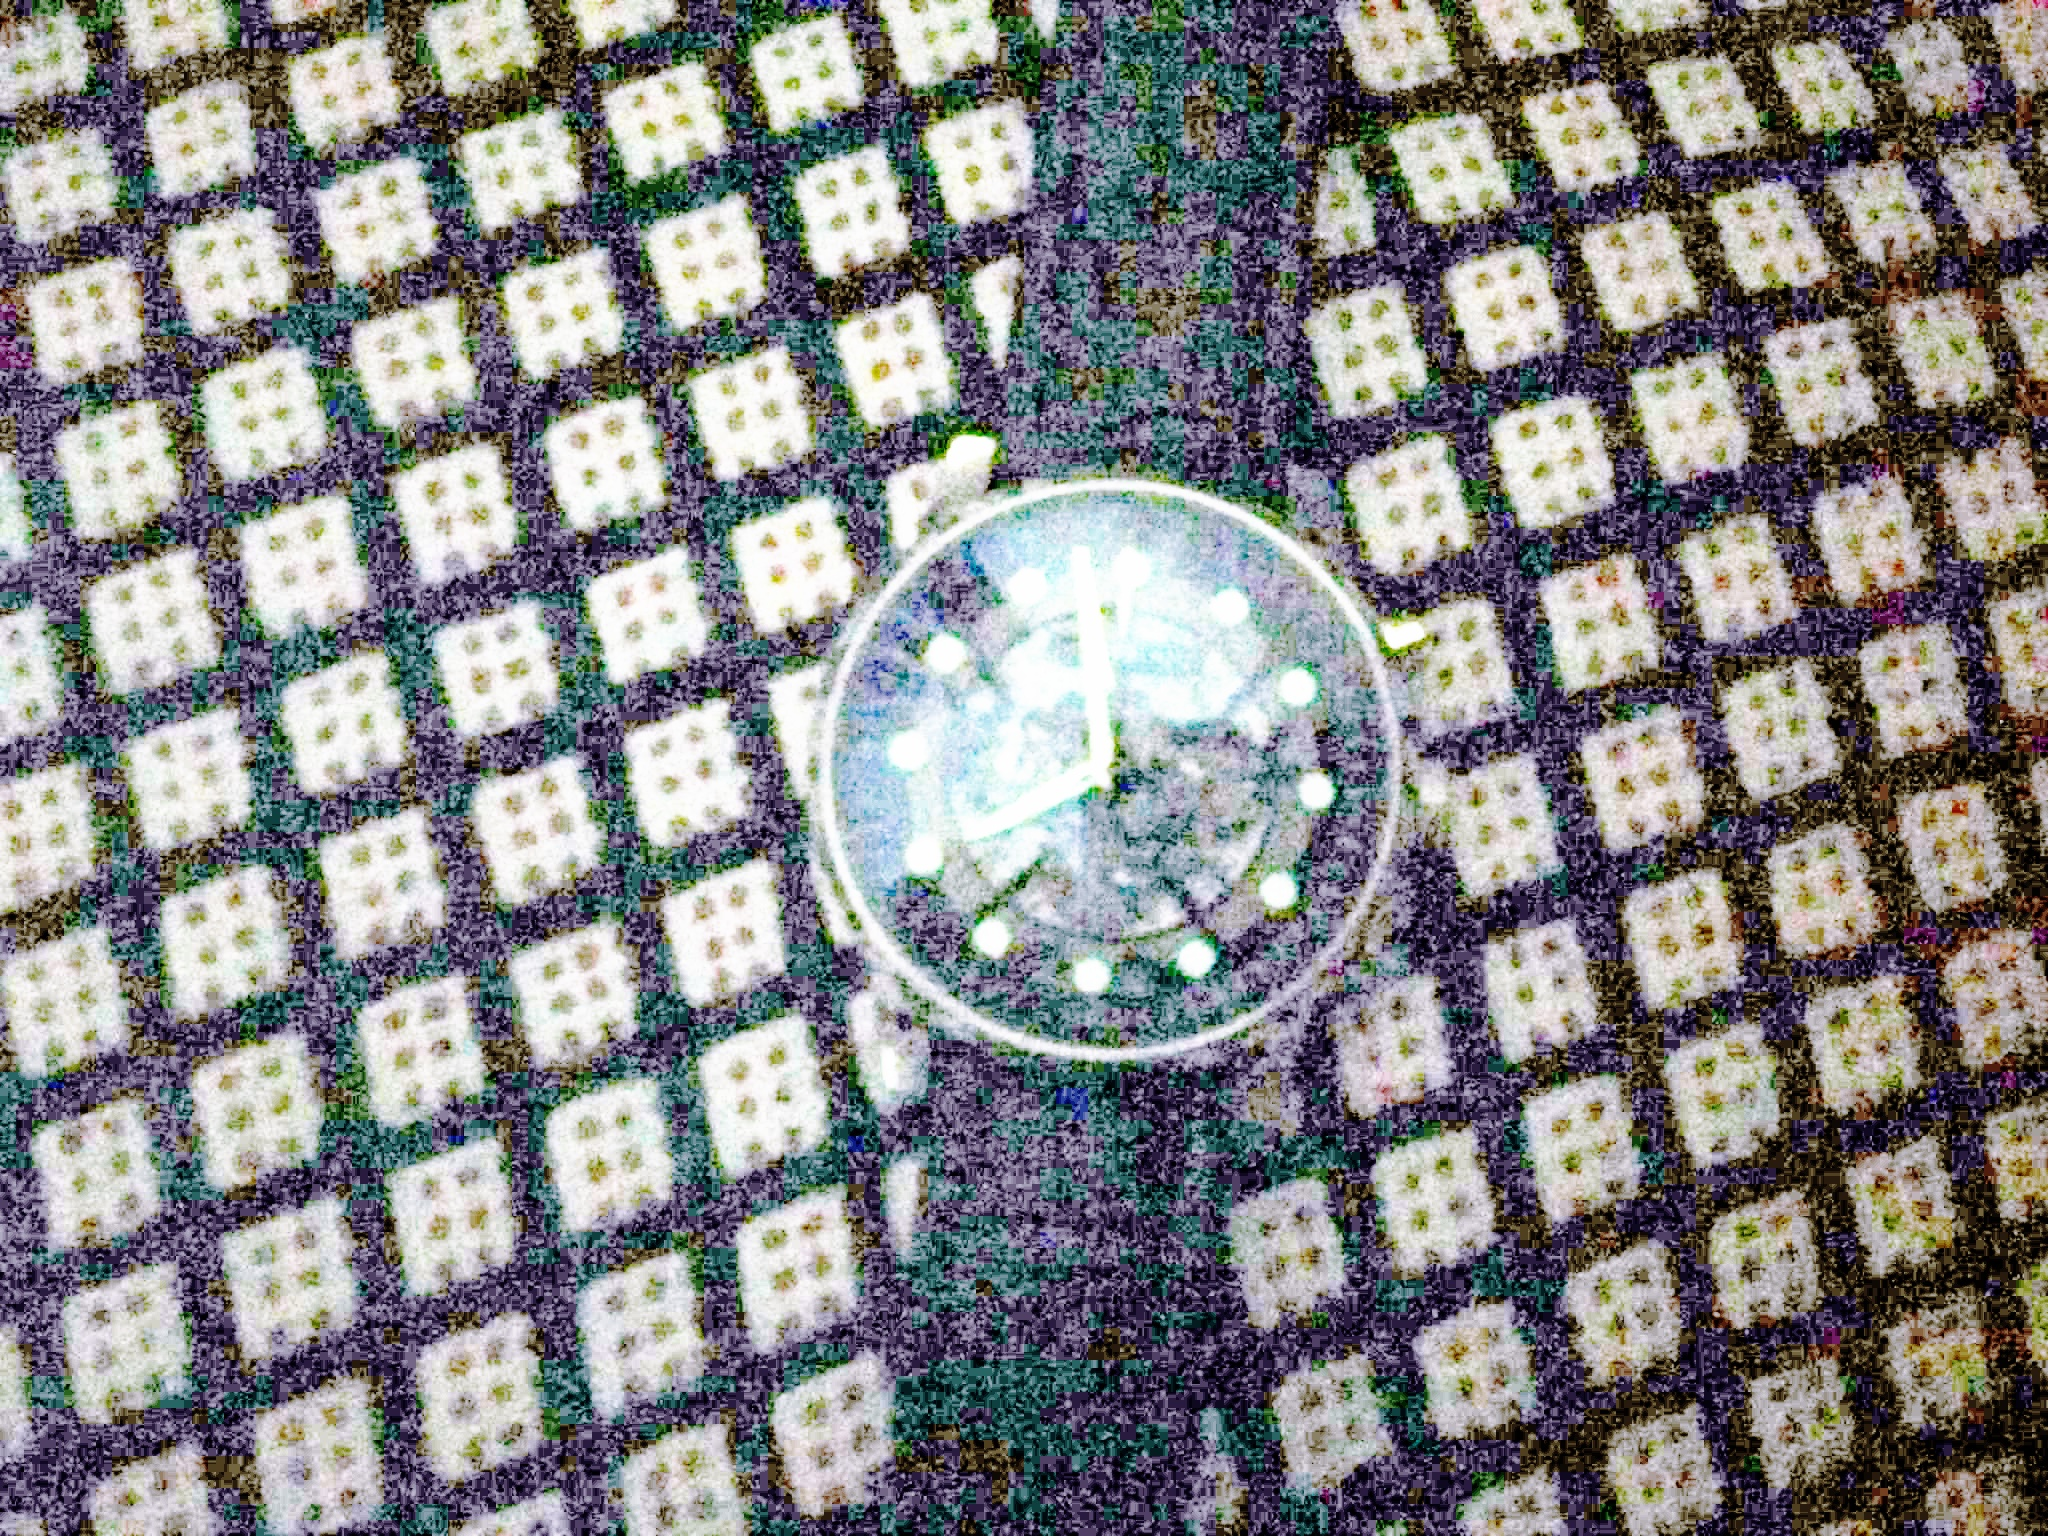
\includegraphics[width=\textwidth]{result_watch.jpg}
    \caption{Adaptive histogram equalized image}
    \label{fig:result_lena}
  \end{subfigure}
  \caption{The entropy of image in left is [4.34354707,4.54178776,4.45467984] and for image in right is [ 7.6624134,7.22025791,7.45981443] in [B,G,R] sequence.}
\end{figure}

\clearpage
\newpage
\subsection{Contrast Limited Adaptive Histogram Equalization}

\par
Conventional histogram equalization operates by aiming to equalize the histogram of entire image \emph{i.e} global contrast of the image is considered. This technique yields good result if the contrast of the image is uniform or nearly uniform over the entirety of the image. However, if the image has regions of sharp difference in contrast, then this technique will usually result in blowing up of detail in bright areas. Contrast Limited Adaptive Histogram Equalization (CLAHE) was developed to address this issue.
\par
Open CV provides pre-built functions for performing CLAHE. The approach used by Open CV is discussed here. In this, image is divided into smaller blocks called \emph{"tiles"} (tileSize is 8x8 by default in OpenCV). For each tile, histogram equalization is performed using conventional technique. If there is presence of noise or outliers;identified as points having aberrant value from its neighbors, the effect of noise is amplified. So, in order to avoid this problem, \emph{contrast limiting} is applied. If any histogram bin is above preset limit, these pixels are clipped and the surplus value is uniformly distributed to other bins before applying histogram equalization. Bilinear interpolation is applied at the end to remove artifacts tile borders.

\subsubsection{Results}


\begin{figure}[!h]
  \begin{subfigure}[b]{0.3\textwidth}
    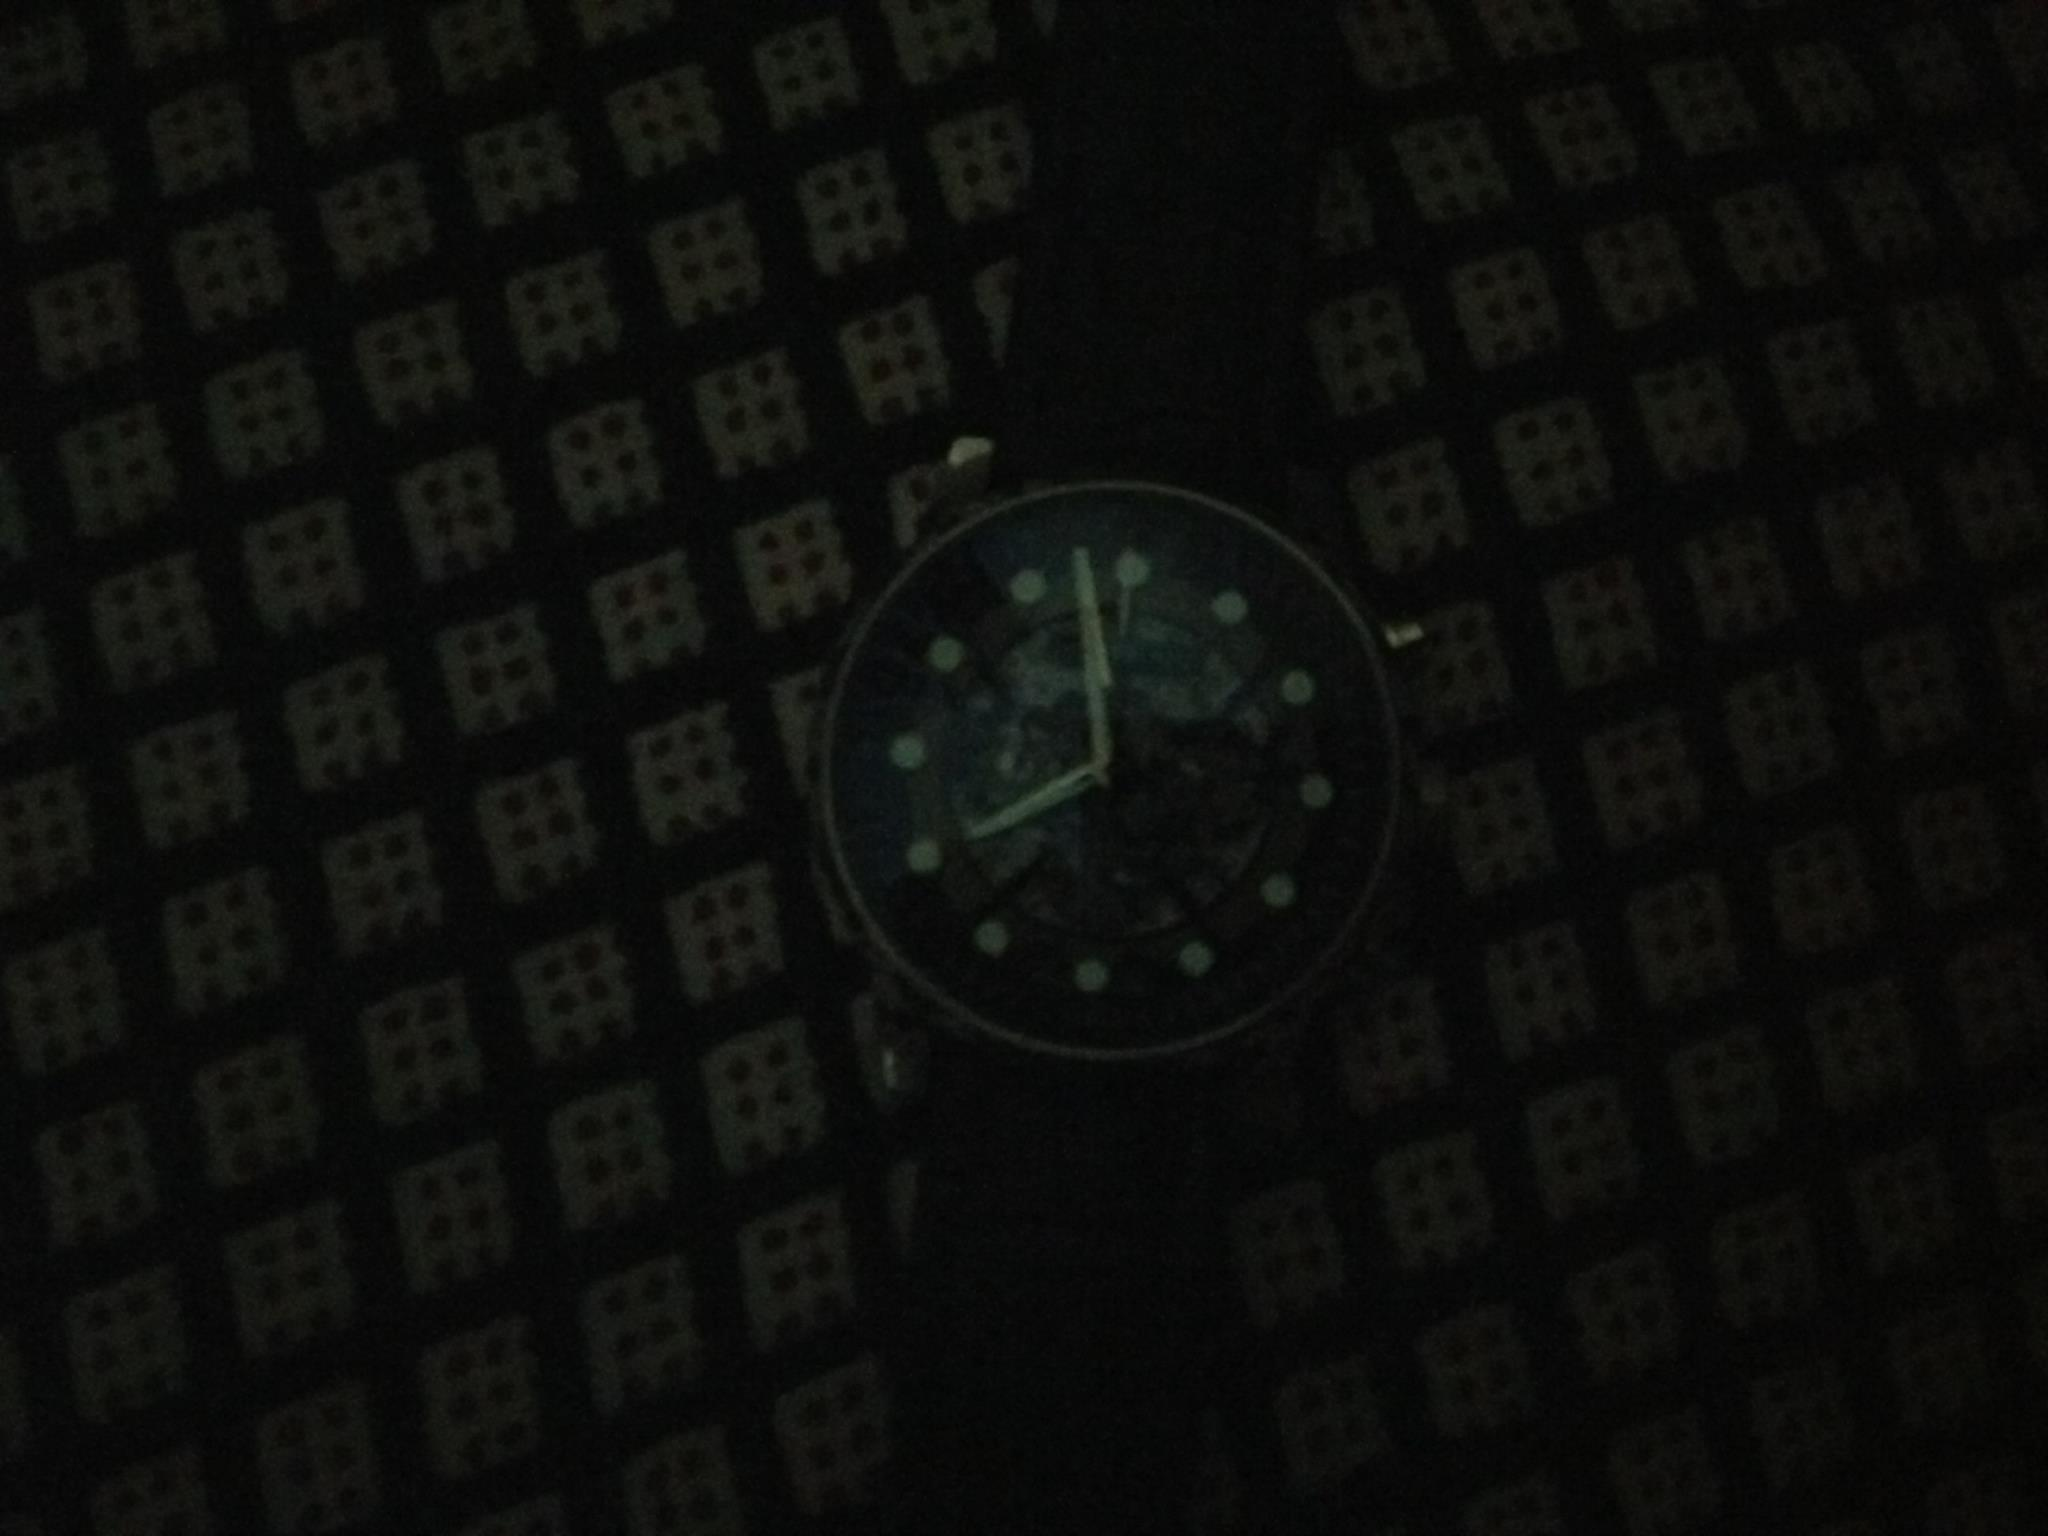
\includegraphics[width=\textwidth]{watch.jpg}
    \caption{Original Image}
    \label{fig:orig}
  \end{subfigure}
  \begin{subfigure}[b]{0.3\textwidth}
    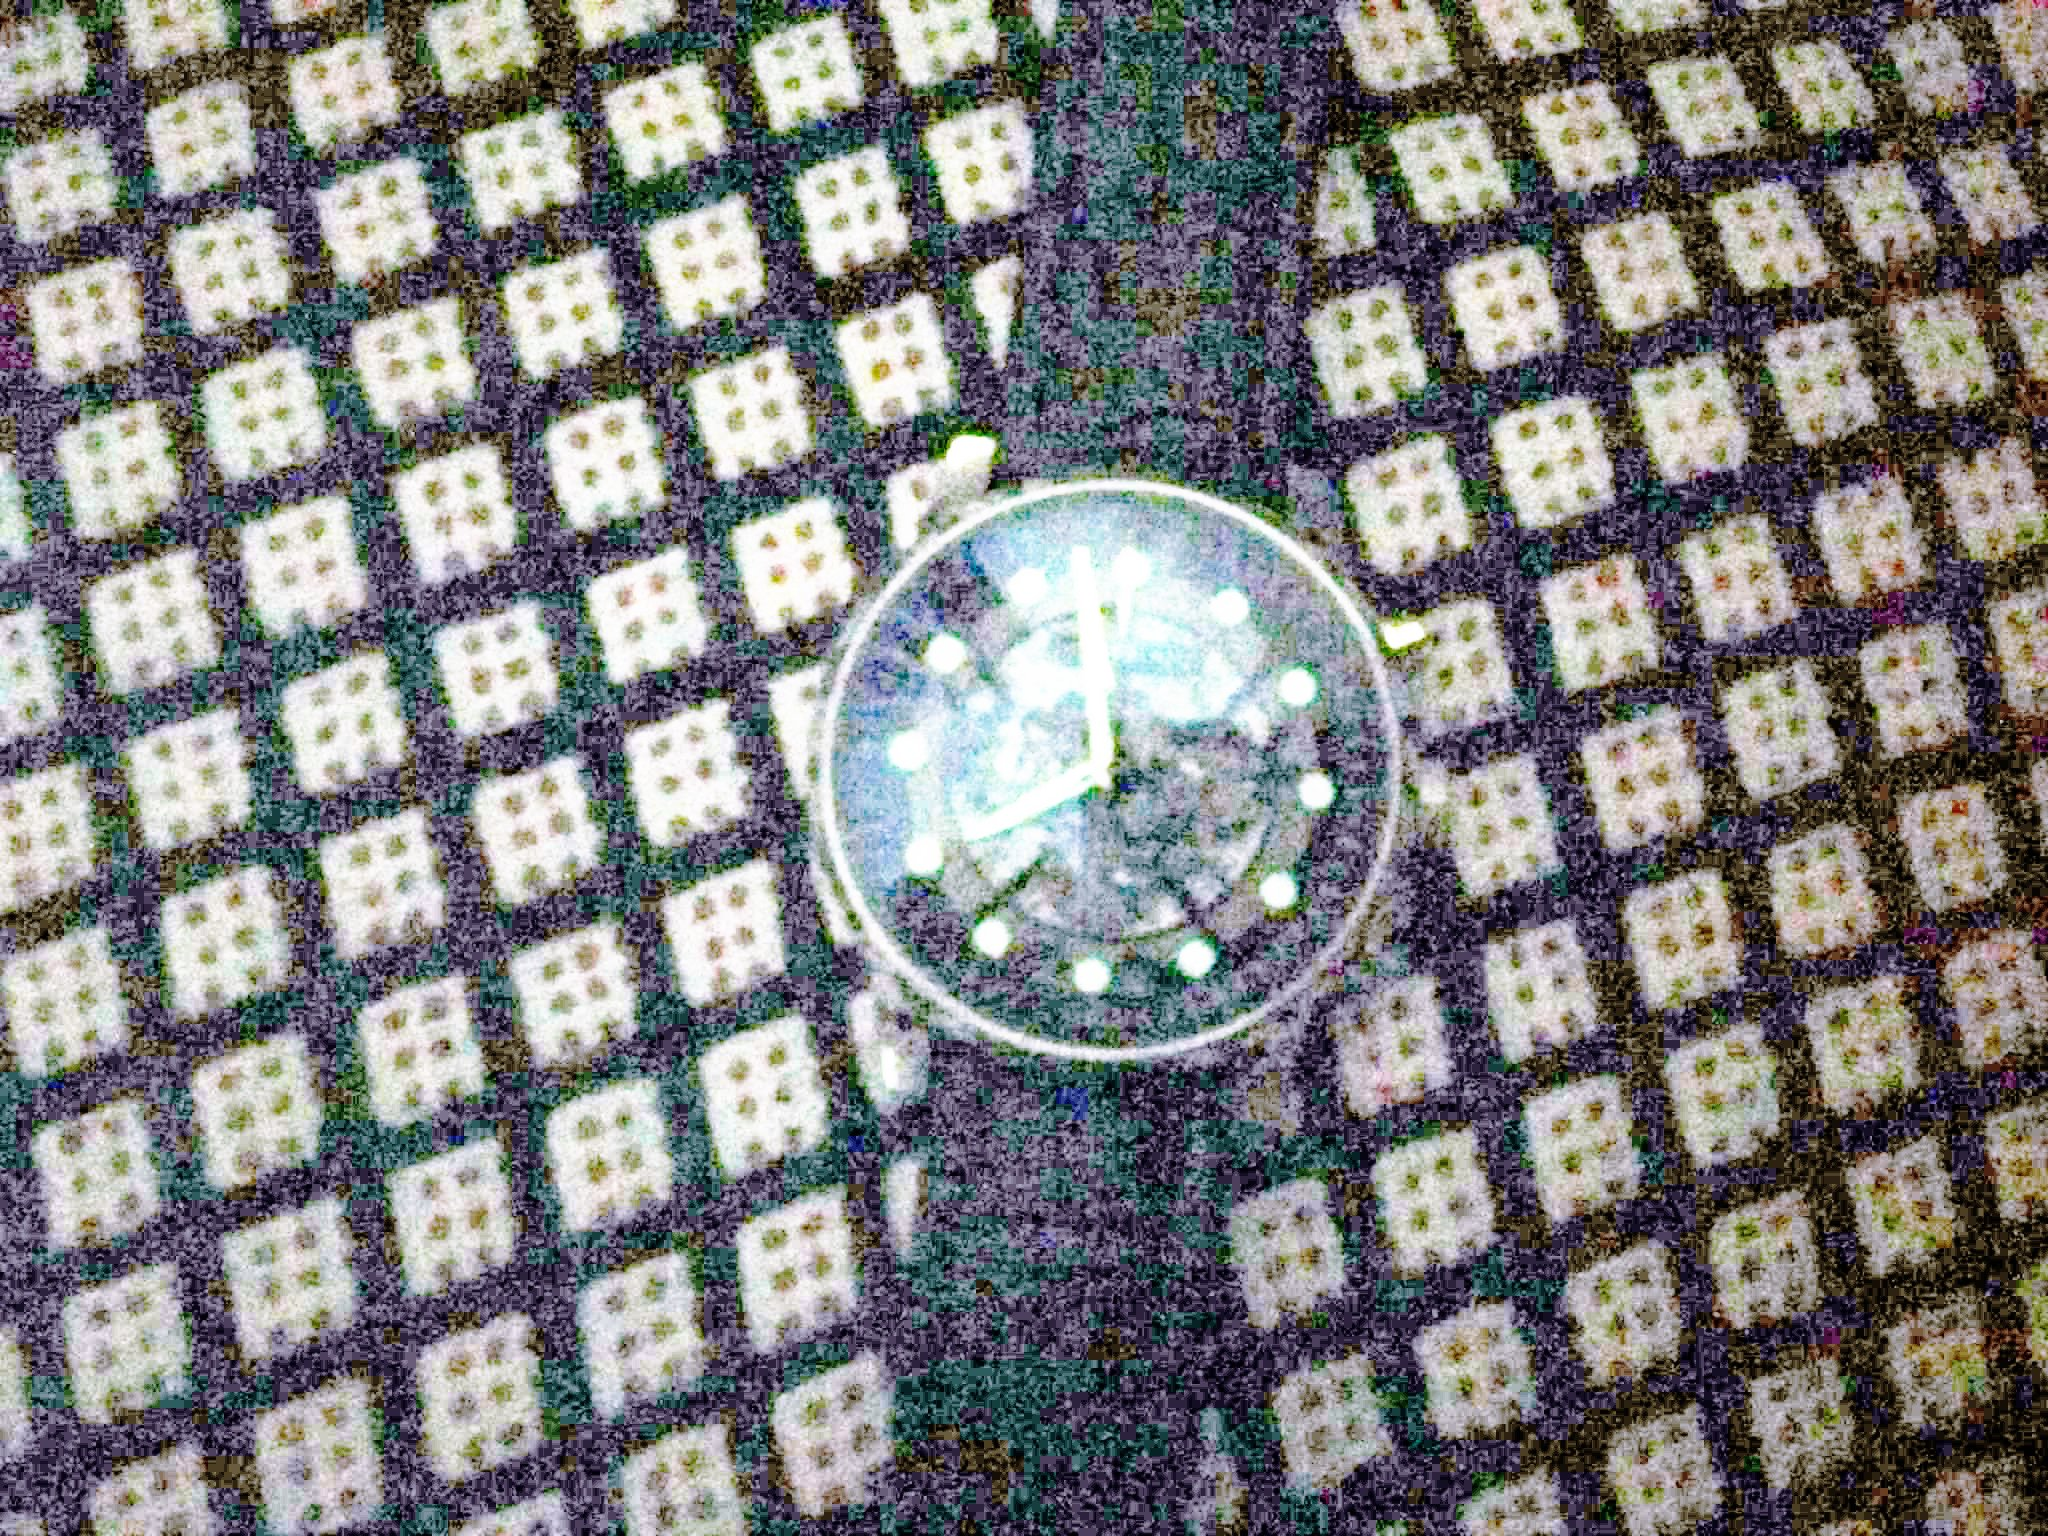
\includegraphics[width=\textwidth]{hist_watch.jpg}
    \caption{traditional method}
    \label{fig:hist_wat}
  \end{subfigure}
   \begin{subfigure}[b]{0.3\textwidth}
    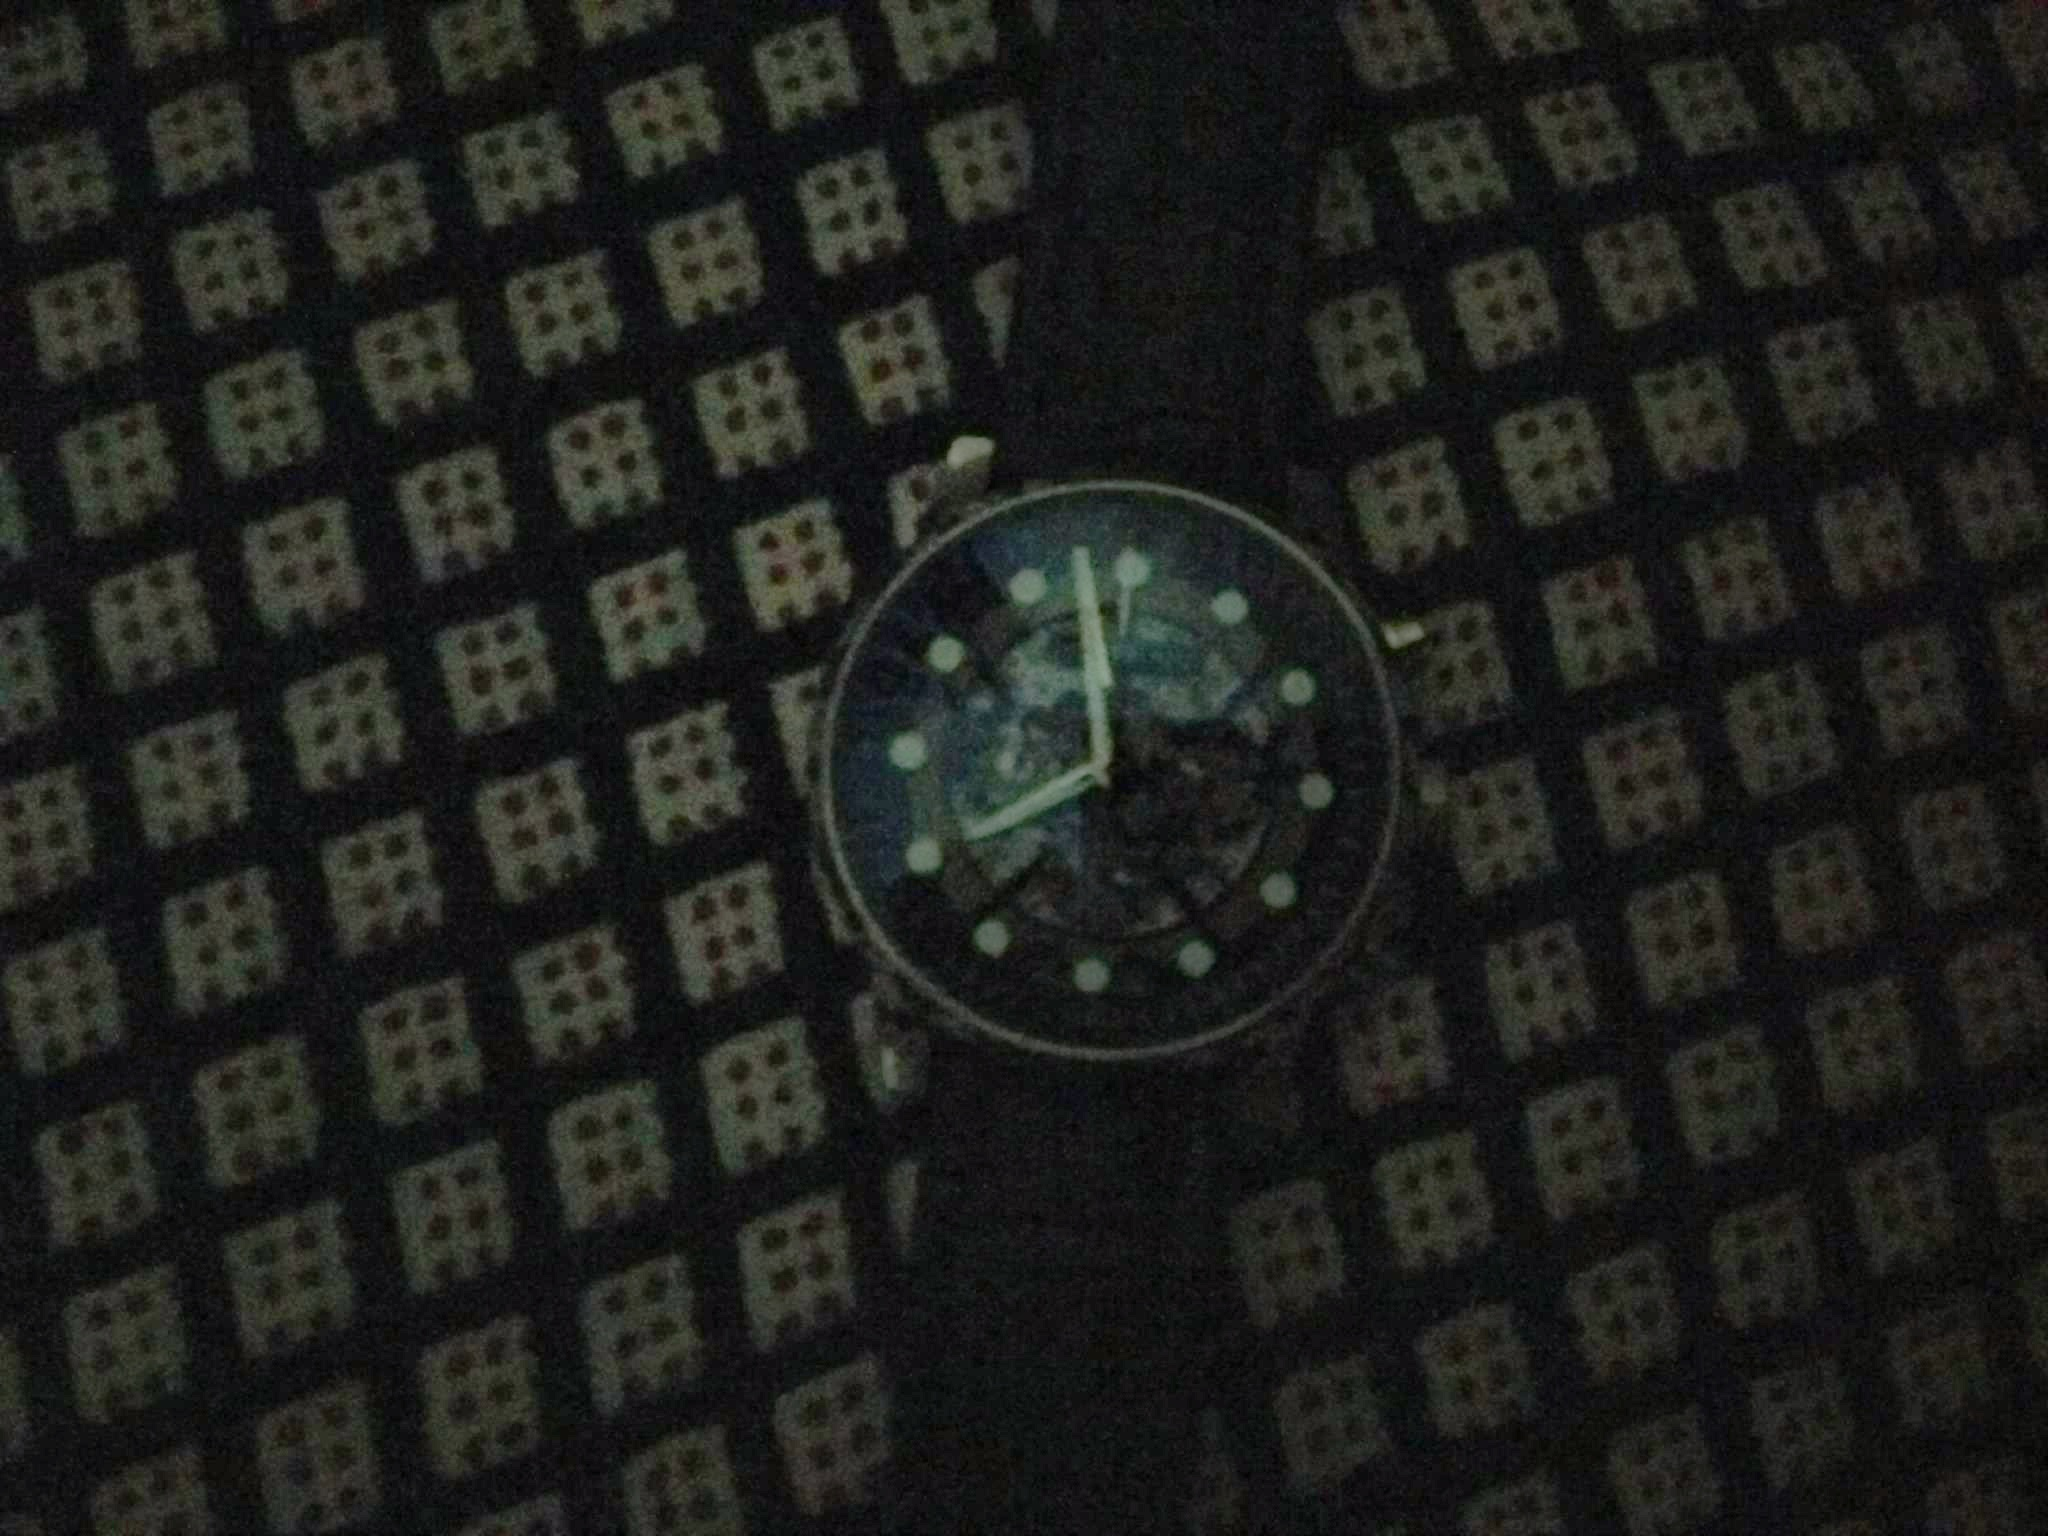
\includegraphics[width=\textwidth]{clahe_watch.jpg}
    \caption{CLAHE Image}
    \label{fig:clahe_watch}
  \end{subfigure}
  \caption{Application of histogram equalization and CLAHE}
\end{figure}











\clearpage
\newpage
\subsection{Automatic Color Enhancement (ACE)}
\par
Automatic Color Enhancement(ACE) is an effective color correction and enhancement method. This method is based on a simple model of the human visual system and based on following low level methods[6]:
\begin{itemize}
	\item "gray world"; average perceived color is gray
    \item "white patch"; normalization is towards a white reference
	\item "lateral inhibition"
    \item "local global adaptation"
\end{itemize}
\par
The combination of these models can simulate perception and image will seem more natural.

\subsubsection{Algorithm}

%\begin{enumerate}
\par
Image stored in various formats are read by python modules and stored in an array format. The array is multidimensional and shape being (width, height, depth). Depth refers to the number of color channels. For an RGB image it is 3 and 1 (or absent) for gray-scale.
\par
For input gray-scale image or a chromatic channel of a multi-depth image, operation R(x) is performed on every channel and later combined.

\begin{equation}
R(x) = \sum_{y\epsilon \Omega \backslash x}{\frac{S_\alpha (I(x) - I(y))}{ \mid \mid x - y \mid \mid}}%{\abs{\abx-%y}}} , x \epsilon \Omega
\end{equation}
where $\lbrace\Omega\backslash x\rbrace$ represents $\lbrace y \epsilon \Omega :y\neq x\rbrace$ and denominator gives the Euclidean distance; $S_\alpha : [-1, 1] \to R$ (slope function), $S_\alpha(t) = min\lbrace max\lbrace\alpha t, -1\rbrace, 1\rbrace$ for some $\alpha\geq 1$. 
This is the first stage of ACE method and adapts local image contrast. The neighboring pixel intensity differences are weighted by the inverse of Euclidean distance. The curve of the function $S_\alpha$ is as follows:


\begin{center}
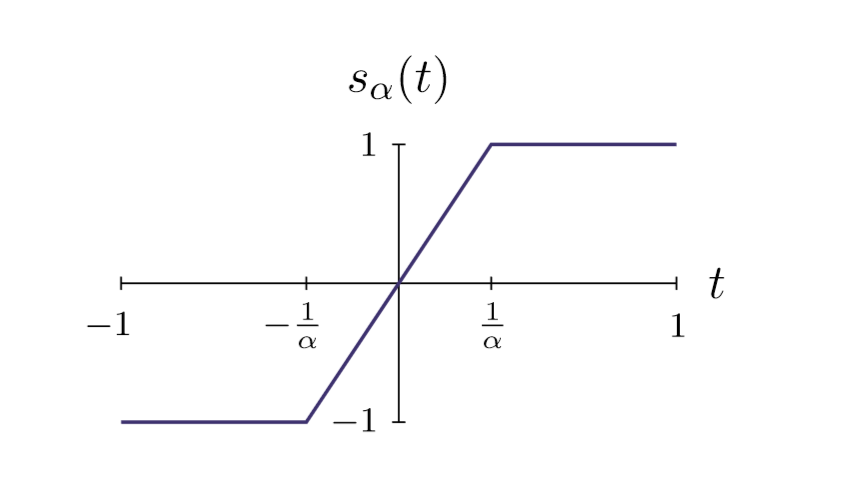
\includegraphics[scale=0.5]{Capture.PNG}
\label{fig:slope_plot}
\captionof{figure}{Slope function plot}
\end{center}

\par
The limit $\alpha$ $\rightarrow$ $\infty$, it is the signum function $s_\infty$ (t) = sign(t). The enhanced channel is then calculated by stretching R to [0,1].

\begin{equation}
L(x) = \frac{R(x) - min R }{man R - min R}
\end{equation}

\par
This is the second stage and adjusts the image to achieve a global white balance. This complete enhancement process is consistent with visual perception. It is shown that adjusting few hyper-parameters like $\alpha \to \infty$, the ACE can be viewed as smoothed and localized variation of Uniform Histogram Equalization. 
\par
ACE can be tweaked by altering:
\begin{itemize}
\item slope function $S_\alpha$
\item weight function
\item windowing of y
\item various normalizations for L
\end{itemize}

%\begin{equation}
%O_c(p) = round [127.5 + s_c R_c(p)] % oii kun formula use gareko?? link pathau ta
%\end{equation}
%\begin{equation}
%M_c = max[R_c [p]]
%\end{equation}
%\begin{equation}
%m_c = min[R_c [p]]
%\end{equation}

%\begin{equation}
%\Delta E_m_e_a_n = \frac{\sum_{x=0}^{size x}\sum_{y=0}^{size y} \Delta E(I_1(x,y),I_2(x,y))}{N}
%\end{equation}

%\end{enumerate}


\subsubsection{Results}

\begin{figure}[!h]
  \begin{subfigure}[b]{0.3\textwidth}
    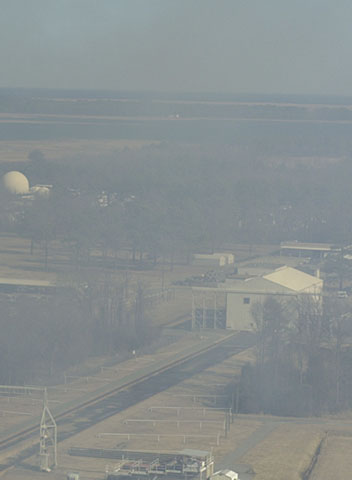
\includegraphics[width=\textwidth]{avs.jpg}
    \caption{Original Image}
    \label{fig:misty}
  \end{subfigure}
  \begin{subfigure}[b]{0.3\textwidth}
    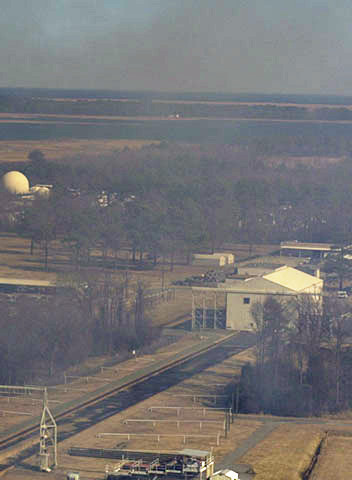
\includegraphics[width=\textwidth]{123.jpg}
    \caption{ACE enhancement}
    \label{fig:ace}
  \end{subfigure}
   \begin{subfigure}[b]{0.3\textwidth}
    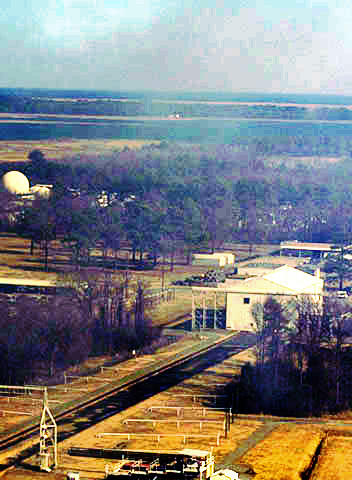
\includegraphics[width=\textwidth]{hist.jpg}
    \caption{Histogram equalized}
    \label{fig:hist_scene}
  \end{subfigure}
  \caption{Application of automatic color enhancement}
\end{figure}









\clearpage
\newpage
\nocite{*}
\bibliography{references} 
\bibliographystyle{ieeetr}

\end{document}
